%--------------------
% Packages
% -------------------
\documentclass[11pt,a4paper]{article}
\usepackage[utf8x]{inputenc}
\usepackage[T1]{fontenc}
%\usepackage{gentium}
\usepackage{mathptmx} % Use Times Font
\usepackage[pdftex]{graphicx} % Required for including pictures
\usepackage[pdftex,linkcolor=black,pdfborder={0 0 0}]{hyperref} % Format links for pdf
\usepackage{calc} % To reset the counter in the document after title page
\usepackage{enumitem} % Includes lists
\frenchspacing % No double spacing between sentences
\linespread{1.2} % Set linespace
\usepackage[a4paper, lmargin=0.1\paperwidth, rmargin=0.1\paperwidth, tmargin=0.05\paperheight, bmargin=0.05\paperheight]{geometry} %margins
%\usepackage{parskip}
\usepackage[all]{nowidow} % Tries to remove widows
\usepackage[protrusion=true,expansion=true]{microtype} % Improves typography, load after fontpackage is selected
\usepackage{lipsum} % 
\usepackage{caption}
\usepackage{subcaption} % Used for inserting dummy 'Lorem ipsum' text into the template
% \usepackage{subfigure} % Used for inserting dummy 'Lorem ipsum' text into the template
%-----------------------
% Set pdf information and add title, fill in the fields
%-----------------------
\hypersetup{ 	
pdfsubject = {},
pdftitle = {},
pdfauthor = {}
}

\renewcommand{\t}[1]{\texttt{#1}}
\renewcommand{\b}[1]{\textbf{#1}}
\renewcommand{\i}[1]{\emph{#1}}
\usepackage{listings}
\usepackage{xcolor}

% Color definition
\definecolor{codegray}{rgb}{0.3,0.3,0.3}
% \definecolor{black}{rgb}{0,0,0}

% Listings configuration
\lstdefinestyle{BugHunterExact}{
    basicstyle=\ttfamily\small\linespread{0.9}\selectfont, % slightly reduce line spacing
    keywordstyle=\bfseries,
    commentstyle=\itshape\color{codegray},
    numbers=none,
    numberstyle=\scriptsize\ttfamily\color{black},
    numbersep=8pt,
    numberblanklines=false,
    frame=tb,
    framerule=0.5pt,
    rulecolor=\color{black},
    escapeinside={(*@}{@*)},
    captionpos=b,
    abovecaptionskip=8pt,
    belowcaptionskip=4pt,
    xleftmargin=0pt, % Fixes unwanted indentation
    xrightmargin=0pt,
    columns=fullflexible,
    tabsize=4,
    keepspaces=true,
    lineskip=0pt, % reduce line spacing
    showstringspaces=false,
    breaklines=true,
    breakatwhitespace=true,
}


% Custom caption style
\DeclareCaptionFormat{listing}{
  \normalfont \textbf{#1:}~#3 
}
\captionsetup[lstlisting]{format=listing,singlelinecheck=false,labelfont=bf}

%-----------------------
% Begin document
%-----------------------



\begin{document} 

{\Large \textbf{CGGS-CW2 Report}}\\
\indent \indent {\large s2150204}

\subsection*{Section 1-2 Observations}

This report evaluates the performance of linear FEM for soft-body simulation, where deformations arise solely from initial velocity impulses without external forces. 
All scenes that are referred to can be found in \texttt{<submission>/videos/<scene>.mp4}.

In the bunny scene, a model with low initial deformation behaves as expected. The overall deformation remains minimal, with only a slight oscillation of the ears until the system stabilizes. This result confirms that linear FEM works well when deformations are small and that no significant artifacts occur under these conditions.

The cube scene tests two cubes with different material stiffness under medium initial deformation. The compliant cube deforms more noticeably than the stiff one, and although both resolve their deformations, a slight rotation, flattening, and expansion are observed afterward. These outcomes align with predictions: while linear FEM resolves the deformation, its linear approximation introduces predictable artifacts in moderate deformation scenarios.

In the epcot scene, where a high initial deformation is applied, the object flattens and expands as it relaxes. Despite the pronounced deformation, the method successfully brings the system to a resolved state. However, the observed flattening and expansion confirm that linear FEM struggles to accurately capture the behavior under large deformations.

The fertility scene features two instances of the same mesh with differing initial deformations. As anticipated, the instance with high initial deformation exhibits significant early distortion, whereas the low-deformation instance remains relatively stable. Both eventually settle into a resolved configuration, demonstrating that the initial conditions strongly influence the simulation outcome.

A newly added torsion scene further illustrates the method’s behavior. In this scene, a box is subjected to a torsional impulse that causes it to twist. As a result, the box expands along the axis of rotation. This expansion is a predictable artifact of the linear approximation when handling torsional loads, reinforcing the observation that, while linear FEM is efficient and stable, it may not fully capture the complex behavior associated with rotational deformations.

In conclusion, these simulations confirm that linear FEM is computationally efficient and produces stable, plausible results for small to moderate deformations. However, for larger deformations, predictable artifacts such as rotation, flattening, and expansion emerge. These effects are inherent in the linear approximation, suggesting that alternative approaches like the corotational method should be considered when higher accuracy is required under large deformations.



\subsection*{Extension}

\subsubsection*{Implementation}

My implementation of corotational elements consisted of a tweak to the \texttt{create\_element\_stiffness} function I had previously implemented, and a tweak to the \texttt{update\_scene} function. 
Starting with the scene class, when the scene is updated the large scene FEM matrix is reinitialised, and then the solver is factorised. 
This follows almost the exact same steps as the original scene file, but without initialisation steps. 
Then, in the mesh class, the code shown in Listing \ref{lst:extra} is added after $K_{e}$ is initialised.
This directly implements the lecture slides into code, and then transforms each $K_{e}$ individually.
\begin{lstlisting}[language=C++, style=BugHunterExact, caption={Source file: \t{mesh\_section3.h}, Function: \t{create\_element\_stiffness()}}, label={lst:extra}]
[..]
138   // ======= Corotational Element ========
139
140   // Construct stacked matrices P and Q
141   Matrix<double,3,3> P, Q;
142
143   for (int i = 0; i < 3; i++) {
144     // Original undeformed edges
145     Vector3d x0 = origPositions.segment<3>(3 * tet(0));   // x1
146     Vector3d xi = origPositions.segment<3>(3 * tet(i+1)); // xn
147     P.col(i) = x0 - xi; 
148            
149     // Current deformed edges
150     x0 = currPositions.segment<3>(3 * tet(0));   // x1'
151     xi = currPositions.segment<3>(3 * tet(i+1)); // xn'
152     Q.col(i) = x0 - xi;
153   }
154 
155   // Compute rotation matrix S and use SVD to get R 
156   Matrix3d S = P.transpose() * Q;
157   JacobiSVD<Matrix3d> svd(S, ComputeFullU | ComputeFullV);
158   Matrix3d R = svd.matrixV() * svd.matrixU().transpose();
159         
160   // Ensure R is a rotation (det(R) positive)
161   if (R.determinant() < 0.0) {
162     Matrix3d V = svd.matrixV();
163     V.col(2) *= -1.0;
164     R = V * svd.matrixU().transpose();
165   }
166 
167   // Construct the larger rotational element so it applies it to all 
168   //  vertices within the tet
169   Matrix<double, 12, 12> Re = Matrix<double, 12, 12>::Zero();
170   for (int i = 0; i < 4; ++i) {
171     Re.block<3,3>(3*i, 3*i) = R;
172   }
173   // Corotational stiffness matrix (from lecture slides: K' = R*K*R^-1)
174   // R tranpose is the same as the inverse 
175   Matrix<double, 12, 12> Ke_corot = Re * Ke_linear * Re.transpose();
176 
177   return Ke_corot.sparseView();
[..]
\end{lstlisting}


\subsubsection*{Observations}

We can see the benefits afforded by the co rotational element in a variety of scenes. 
Figure~\ref{fig:comparison-deformation} shows a sequence of comparisons before and after the co rational element was added. 
Figure~\ref{subfig:deform-epcot} shows the difference at frame 25 of the Epcot scene before and after the co rotational element was added. 
Figure~\ref{subfig:deform-cube86} shows a similar difference at frame 25 the cube86 scene. 
In both scenes the objects initially deform and then slowly tilt and expand outwards in the original implementation.
In the updated implementation, the objects instead deform and then resolve correctly. 
This is due to rotations being present in the deformation. 
When the linear system is used, it cannot account for rotational deformation, so the inconsistencies with the deformation add up. 
This leads to artifacts such as these.
In comparison, when rotational elements are taken into account, these scenes correctly deform, and resolve correctly. 

\begin{figure}[t]
  \centering
  \begin{subfigure}[b]{0.6\textwidth}
    \centering
    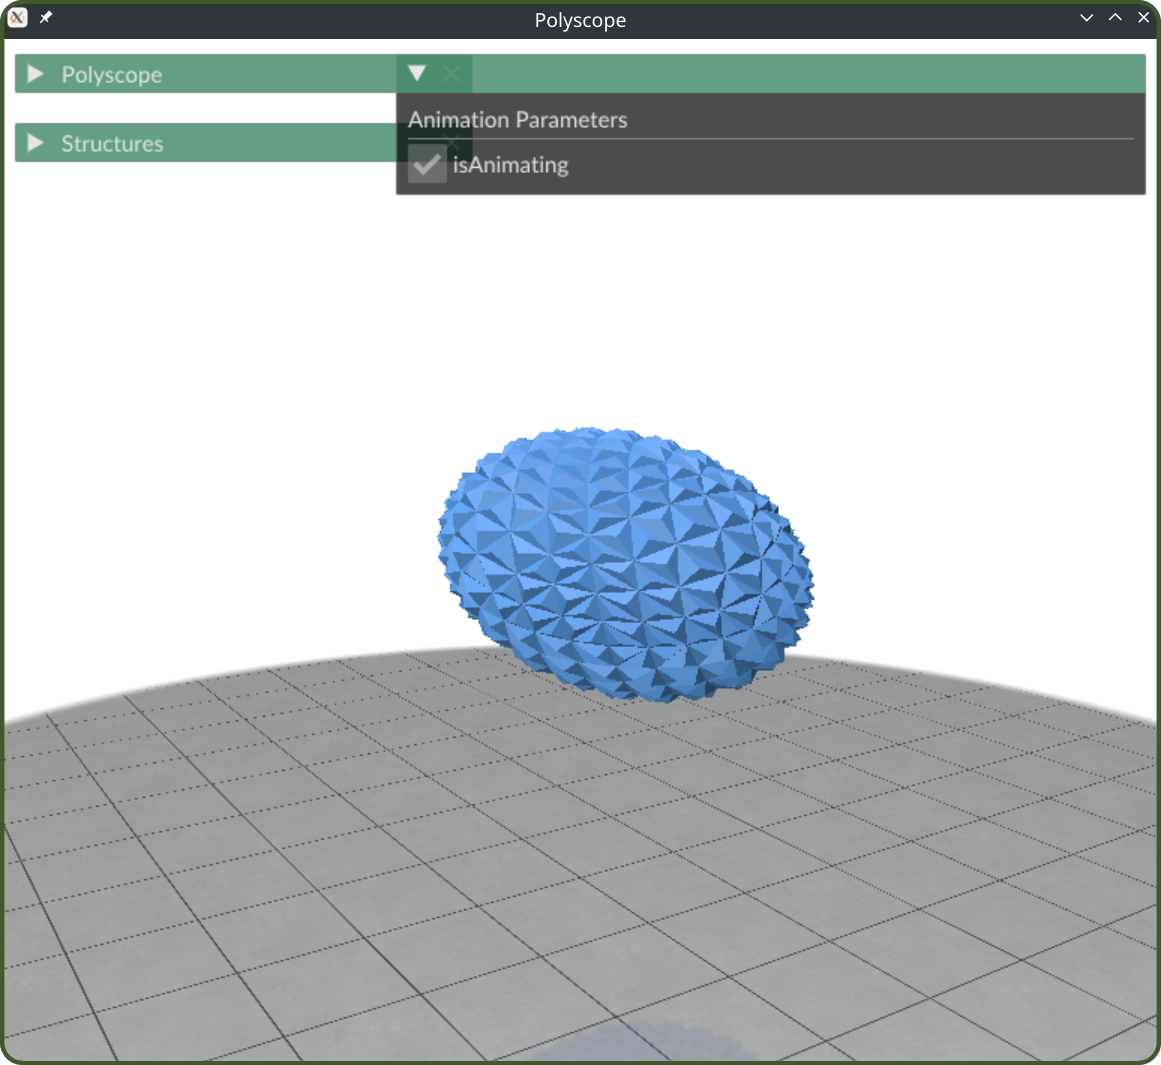
\includegraphics[width=0.5\textwidth]{figures/epcot-linear.png}%
    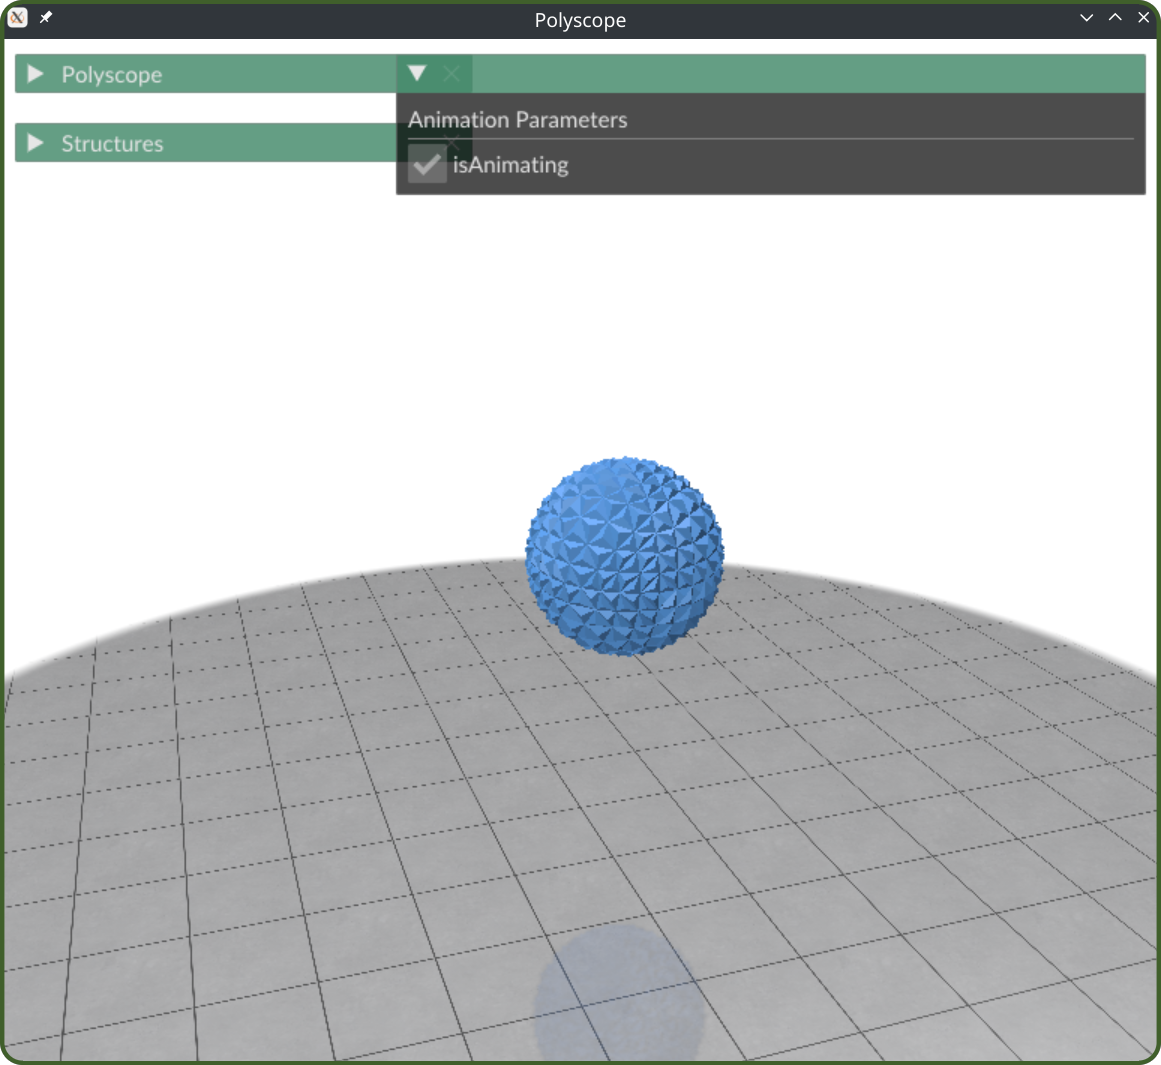
\includegraphics[width=0.5\textwidth]{figures/epcot-corot.png}
    \caption{Epcot scene with and without the corotational element. On the left is the linear system and on the right is the corotational system}
    \label{subfig:deform-epcot}
  \end{subfigure}% 
  \hfill
  \begin{subfigure}[b]{0.6\textwidth}
    \centering
    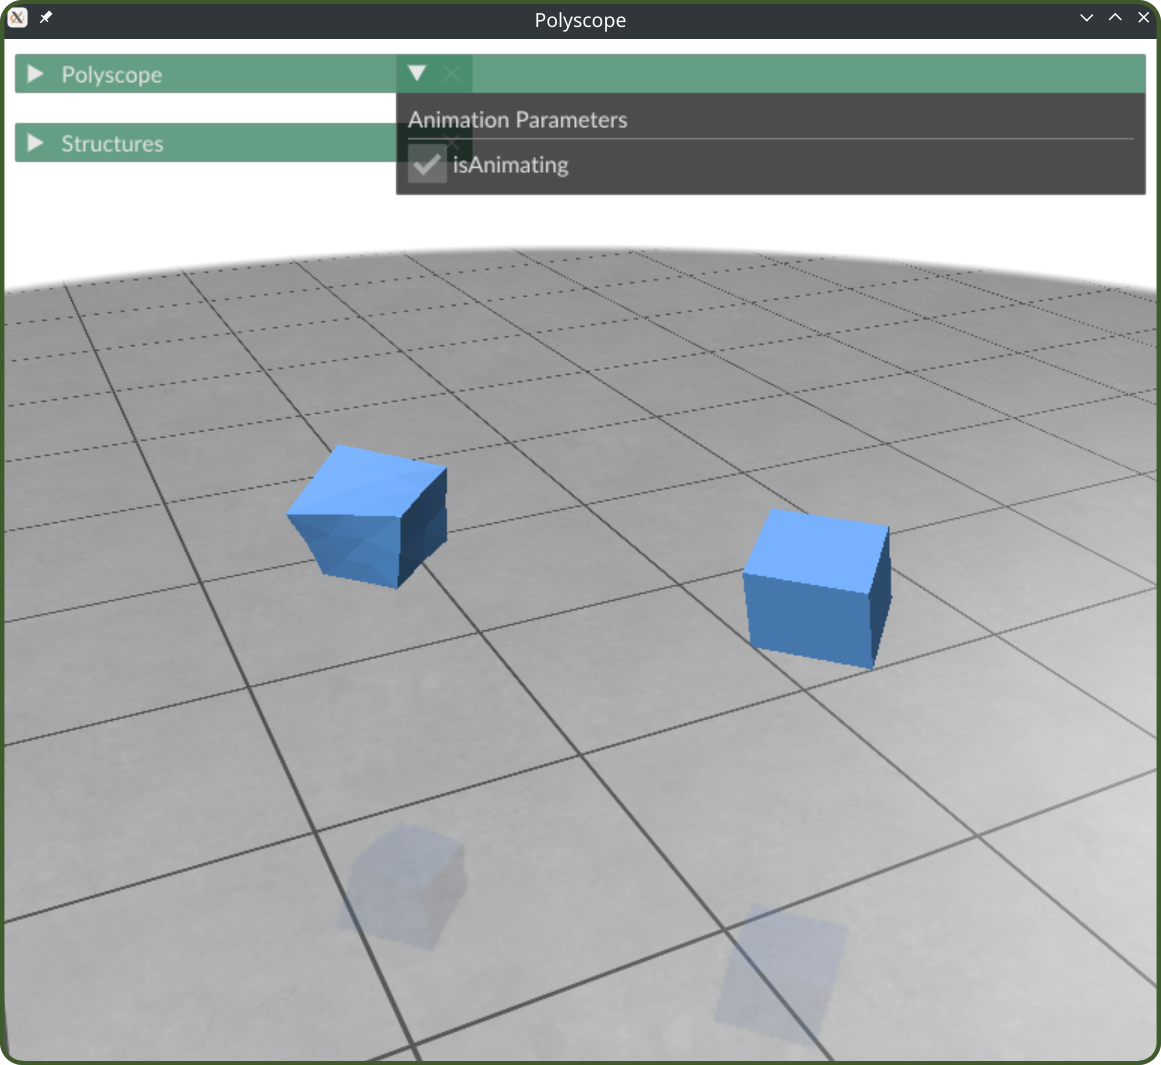
\includegraphics[width=0.5\textwidth]{figures/cube86-linear.png}%
    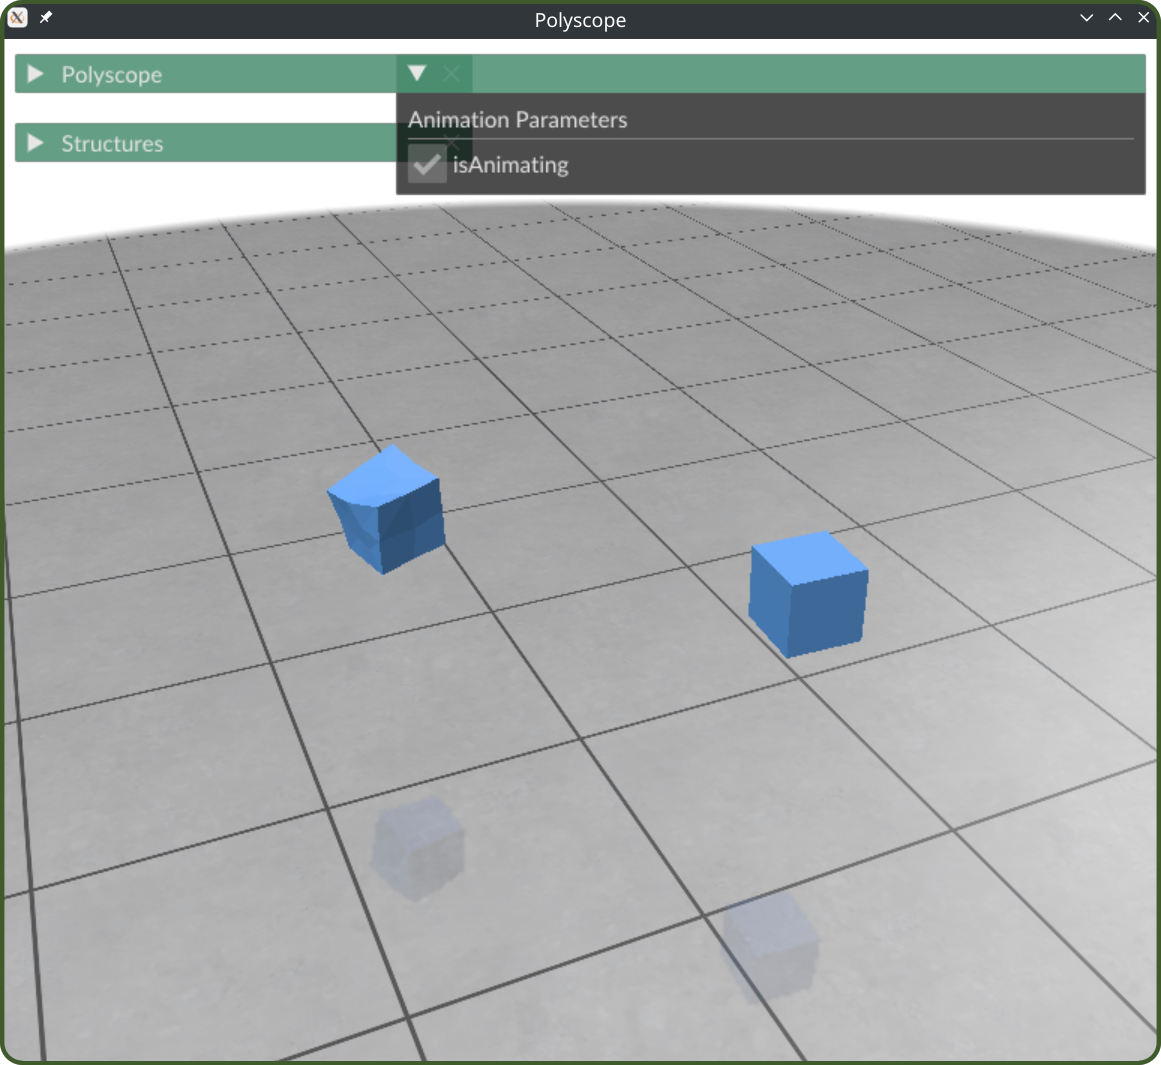
\includegraphics[width=0.5\textwidth]{figures/cube86-corot.png}
    \caption{Cube86 scene with and without the corotational element. On the left is the linear system and on the right is the corotational system}
    \label{subfig:deform-cube86}
  \end{subfigure} 
  \caption{Comparison with and without the corotational element}
  \label{fig:comparison-deformation}
\end{figure}

Despite these benefits, the improvements come with a marked cost. 
The performance on most scene falls by about x\% after the co rotational element is added. 
This is due to the solver being recomputed each frame, which causes each frame to take more processing power to resolve. 
Moreover, there are still artifacts in some scenes. 
For example the fertility scene deforms massively with and without the co rotational element, leading to an unrealistic simulation. 
This indicates that improvements can still be made to this method of soft-body simulation to make it more realistic. 



\end{document}
